\documentclass[dvipdfmx,12pt]{beamer}

\usepackage{bxdpx-beamer}
\usepackage{pxjahyper}
\usepackage{minijs}
\usetheme{AnnArbor}
\usepackage{mathpazo}
\usepackage{amsmath,amssymb}
\usepackage{graphicx}
\usepackage{array}
\usepackage{tikz}
\usepackage{wrapfig}
\usepackage{float}
\usepackage{here}
\setbeamertemplate{navigation symbols}{}

\title{Quantifying Loss-Averse Tax Manipulation}
\subtitle{Alex Ress-Jones}
\author{Reviewd by Reio TANJI}
\date{Nov 13th, 2018}
\institute{Osaka University}

\begin{document}
\begin{frame}\frametitle{}
\titlepage
\end{frame}

\small

\section{Introduction}
\begin{frame}\frametitle{Abstract}
  Alex Rees-Jones (2018)
  ``Quantifying Loss-Averse Tax Manipulation''
  \textit{Review of Economic Studies (2018) 85, 1251–1278}

  \begin{itemize}
    \item Presents the effects of \textit{loss-aversion} from the evidence of
    US taxpayers.

    \item Taxpayers are engaged to persue tax reduction activity especially
    when they have some positive due near the date of payment.

    \item Distribution of reported tax bill has excess mass around the border
    whether they must pay or not.
  \end{itemize}
\end{frame}

\begin{frame}\frametitle{Institutional Background}
  \begin{itemize}
    \item In the US, one's tax payment in each year is determined by the
    Internal Revenue Service (IRS), based on the difference between the
    reported taxable income and the her/his payment in advance:
    ``balance due.''

    \item If the balance due (denoted by $b$) is positive, the tax filer must
    that amount to the IRS, and if negative, then s/he can receive a refund.

    \item Balance due can be ``manipulated,'' by reporting donation they did,
    or enrollment in charitable contribution.

    $\Rightarrow$ Loss-Averse affects the tax filers' behavior according to
    their initial balance due, resulting in the bunching of the reported
    (observed) payment.

  \end{itemize}
\end{frame}

\begin{frame}\frametitle{contribution}
  This paper contributes in three ways:

  \begin{enumerate}
    \item Illustrate robust and observable features of the presence of loss-
    aversion with minimal assumptions.

    \item Estimate the impact of loss-aversion measured in dollers.

    \item Specify the way to apply similar settings:

    loss-averse individual is able to manipulate an observable outcome.
  \end{enumerate}
\end{frame}

\begin{frame}\frametitle{Procedure of the Manipulation}
  Every April, taxpayers go through the process below:
  \begin{enumerate}
    \item Report their taxable income, such as wages, salaries,
    tips, business income, investment income, and so on.

    \item Report ``adjustments,'' to claim for things such as donations or
    payments for alimony

    $\Rightarrow$ Adjusted Gross Income (AGI) is calculated: balance due
    before manipulation.

    \item Accept AGI or complete an additional form of reduction: Itemization

    --Report deductable activities such as charitable contributions, medical
    and dental expenses, home mortgage interest payments.

    \item Final balance due is confirmed:

    Claim credits for pursuing tax incentivised behaviour and report other
    taces paid, payments already made to IRS .
  \end{enumerate}
\end{frame}

\section{Framework}
\begin{frame}\frametitle{Sequential Manipulation}
  \begin{itemize}

    \item Given $b_{\text{PM}}$: balance due prior to manipulation,
    taxpayers face a sequense of manipulation opportunities,
    each of which is charactarized by the parameters
    : $\{ m_i, c_i \} _{i=1} ^{J}$

    $m_i$ denotes the tax reduction by the $i$th manipulation

    $c_i$ is the intrinsic cost

    \begin{block}{Cost by manipulation}
      \footnotesize
      Taxpayers consider their benefits and costs to decide whether to
      make efforts to tax manipulation.

      \begin{itemize}
        \scriptsize
        \item Blumenthel and Slemrod (1992)

        It spend on average 27 hours documenting and reporting for tax
        reduction

        \item Benzarti (2015)

        They dislike tasks for tax 4.2 times as that for working with
        same time length
      \end{itemize}

    \end{block}
  \end{itemize}
\end{frame}

\begin{frame}
  \begin{itemize}
    \item Ordinary gain-loss function:
    \[
    \Phi(x|r) = \begin{cases}
    x-r & \text{ if } x \geq r \\
    \lambda (x-r) & \text{ if } x < r
  \end{cases}
  \]

    \item Applying this structure, loss-averse taxpayers' evaluattion
    of the benefit from each manipulation:

    \begin{align*}
      V(m_i | b, r) &= \Phi(-b + m_i | r) - \Phi(-b | r) \\
       &= \begin{cases}
       m_i & \text{ if } -b \geq r \\
       \lambda(r+b)+(m_i -b -r) & \text{ if } -b \in [r-m_i, r] \\
       \lambda m_i & \text{ if } -b \leq r - m_i
       \end{cases}
    \end{align*}

    \item Taxpayers continue to manipulate iff $m_i < c_i$.
  \end{itemize}
\end{frame}

\begin{frame}\frametitle{Gain-Loss Function}

  \begin{tabular}{cr}
      \begin{minipage}[H]{0.5\textwidth}
        \begin{itemize}
          \item If there remains tax due after reduction, then
          all the value of the manipulation is evaluated as loss.

          \item When, on the other hand, manipulation cancels out the due
          before, the margin to be refunded is evaluated as gain.

          \item If s/he does not have to pay more, then the reduction by the
          manipulation is fully counted as gain.
        \end{itemize}
      \end{minipage} &
      \begin{minipage}[H]{0.5\textwidth}
        \begin{tikzpicture}[domain = -2:2, samples = 200, >= stealth]
          \draw[->] (-2,0) -- (2,0) node[right]{$b$};
          \draw[->] (0,-2) -- (0,2) node[above]{$V(b)$};
          \draw plot[domain = 0:1.7] (\x, {0.6 * \x});
          \draw plot[domain = -1.2:0] (\x, {1.5 * \x});
          \draw (0,0) node [below right] {$r$};
          \draw (0, -2.5) node [below] {gain-loss function};
        \end{tikzpicture}
      \end{minipage}

  \end{tabular}

\end{frame}
\begin{frame}\frametitle{Assumption}
  Assume tax filers consder the most efficient manipulation.

  \begin{itemize}
    \item For $i<j$, $m_i/c_i \geq m_j/c_j$.

    : They considers each oppoturnity of manipulation, in the most efficient
    order.

    \item $m_1/c_1 > 1$.

    : There exists at least one desirable manipulaton oppoturnity.

    \item As $n \to \infty$, $m_n/c_n \to 0$.

    : The number of desirable opportunity is finite.
  \end{itemize}

  Taxpayers continue manipulating as long as $V(m_i|b, r) \geq c_i$,
  and stop when $V(m_i|b, r) < c_i$.
\end{frame}

\begin{frame}\frametitle{Thresholds}
  They define two thresholds of $i \in J$ that stop the manipulation depending
  on the gain-loss situation.

  \begin{align*}
    L &= \max \left \{ i: \dfrac{m_i}{c_i} > 1 \right \} \\
    H &= \max \left \{ i: \dfrac{m_i}{c_i} > \dfrac{1}{\lambda} \right \}
  \end{align*}

  \begin{itemize}
    \item $L$ is the threshold for gain phase, while $H$ is the
     one for loss phase.

     \item $L \leq H$, where equality holds if there is no $i$ s.t.
     $m_i/c_i \in (1/\lambda , 1]$.
  \end{itemize}
\end{frame}
\begin{frame}\frametitle{Example}
  \begin{figure}
    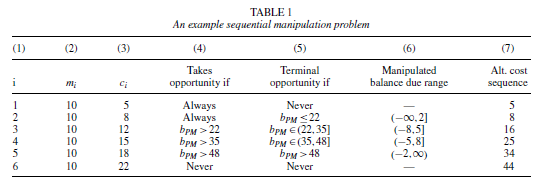
\includegraphics[width = 10cm, height = 4cm]{fig_tab/ARJ_T1.png}
  \end{figure}
  \begin{center}
    $\lambda = 2$
  \end{center}

  When balance initial balance due $b_{PM} \leq 22$, s/he continues
  to manipulate until $i=2$, while one with $b_{PM} > 48$ goes till
  $i = 5$:
  $L = 2, H = 5$.
\end{frame}
\begin{frame}
  \begin{tabular}{ll}
    \begin{minipage}[H]{0.4\textwidth}
      \begin{itemize}
        \item Expected range of the balance due after manipulation is
        $(-8, 8)$, which generates excess mass or bunching.
      \end{itemize}
    \end{minipage} &
    \begin{minipage}[H]{0.5\textwidth}
      \begin{figure}
        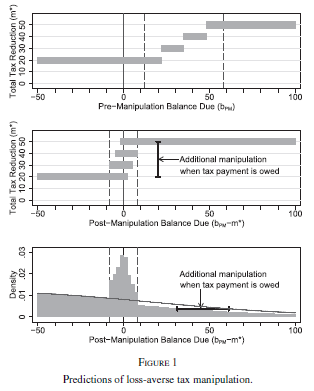
\includegraphics[width = 6cm, height = 8cm]{fig_tab/ARJ_F1.png}
      \end{figure}
      \end{minipage}
  \end{tabular}
\end{frame}
\begin{frame}\frametitle{Total Amount of Manipulation}
  Total manipulation is expressed as a function of the taxpayer's
  pre-manipulation balance due $b_{PM}$:

  \[
  m^* (b_{PM} | r) = \begin{cases}
  \sum _{i=1}^L m_i & \text{ if }b_{PM} \leq T_1 \\
  \sum _{i=1}^{L+1} m_i & \text{ if }b_{PM} \in (T_1, T_2] \\
  \dots \\
  \sum _{i=1}^{L+J-1} m_i & \text{ if }b_{PM} \in (T_{J-1}, T_J] \\
  \sum _{i=1}^{H} m_i & \text{ if }b_{PM} > T_J \\
\end{cases}
  \]
   where $T_j$ denotes

   \[
   T_j = \max \left \{ b_{PM} : V \left( m_{L + j} | b_{PM}
   + \sum_{i=1}^{L+j-1} m_j, r \right) \leq c_{L+j} \right \}
   \]
\end{frame}
\end{document}
